\chapter{Bayesian Classifiers}
  
You drop a net in several places in a lake.   You measure, weigh, and identify every fish to be one of the following 3: \texttt{trout}, \texttt{bass}, or \texttt{catfish}.  Here is a scatter plot of what you find.

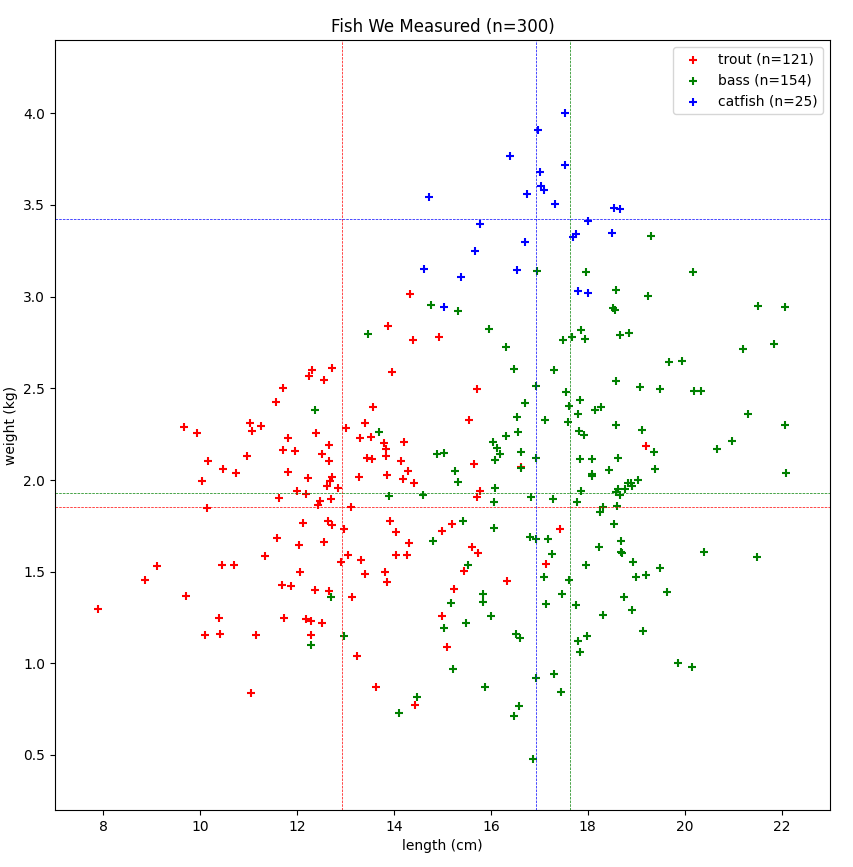
\includegraphics[width=0.7\textwidth]{1_scatter.png}

(Data: \texttt{make\_data.py}, Graph: \texttt{1\_scatter\_fish.py})

The vertical and horizontal lines represent the mean length and width (respectively) of each type of fish.

You are writing a system that someone on the lake could use to identify their fish.

\section{The Prior}

Even before the person measures and weighs the fish,  they can make a decent guess at what any randomly selected fish is:

\begin{tabular}{c | c | c}
Fish & Count & Percent \\
\hline
trout & 121/300 & 40.3\% \\
bass & 154/300 & 51.3\% \\
catfish & 25/300 & 8.3\%
\end{tabular}

If you know nothing about the fish,  there is a 51.3\% chance it is a bass.   The probability without any observations is known as the \textit{prior}:

$$P(\text{fish = trout}) = .403$$
$$P(\text{fish = bass}) = .513$$
$$P(\text{fish = trout}) = .083$$

But, now the user makes an observation: The fish is 16 inches long and weighs 2.1 kg.  Can we update our beliefs based on this? Sounds like a job for conditional probability.

By the definition of conditional probability:

$$P(\text{fish = trout} | \text{length = 16}, \text{weight = 2.1}) = \frac{p(\text{fish = trout} , \text{length = 16}, \text{weight = 2.1}) }{p( \text{length = 16}, \text{weight = 2.1}) }$$

I'm going to run out of space,  so I will use $F$ to represent fish, $L$ to represent length, and $W$ to represent weight.

We can calculate the denominator by summing up all the possibilities.   Now the right-hand side is:

$$\frac{p(\text{F=trout} , \text{L=16}, \text{W=2.1}) }{p(\text{F=trout} , \text{L=16}, \text{W=2.1})  + p(\text{F=bass} , \text{L=16}, \text{W=2.1})  + p(\text{F=catfish} , \text{L=16}, \text{W=2.1})  }$$

We can calculate the probability of all three possibilities (and they will add up to 1.0).

\section{Naive Bayes}

The assumption in naive Bayes is that the probability distributions of length and weight are conditionally independent given the breed of the fish.   That is:

$$p(\text{F=trout} , \text{L=16}, \text{W=2.1}) = p( \text{L=16} | \text{F=trout})  p( \text{W=2.1} | \text{F=trout})P(\text{F=trout})$$

Within a particular species, things like length and weight, which represent of the sum of a lot of genetic and environmental factors,  are often normally distributed.

What if we assume that length has a normal distribution for each kind of fish?  What is the most likely estimator for the mean of each trait?  

$$\mu = \frac{1}{n} \sum_{i=1}^{n} x_i$$

And variance?

$$\sigma^2 = \frac{1}{n} \sum_{i=1}^{n} (\mu - x_i)^2$$

We can compute those pretty easily:

\begin{tabular}{c | c | c | c}
Fish & Trait & $\mu$ & $\sigma^2$ \\
\hline
Trout & Length & 12.91522571 & 3.49054363 \\
 & Weight &1.85290281 & 0.20387574\\
 \hline
Bass & Length & 17.62628327& 4.23881747 \\
 & Weight & 1.92960088&0.45092986 \\
\hline
Catfish & Length &16.92187387 & 1.32301935 \\
 & Weight & 3.42423185 & 0.07244546\\
\end{tabular}

If we plot those probability distributions out:

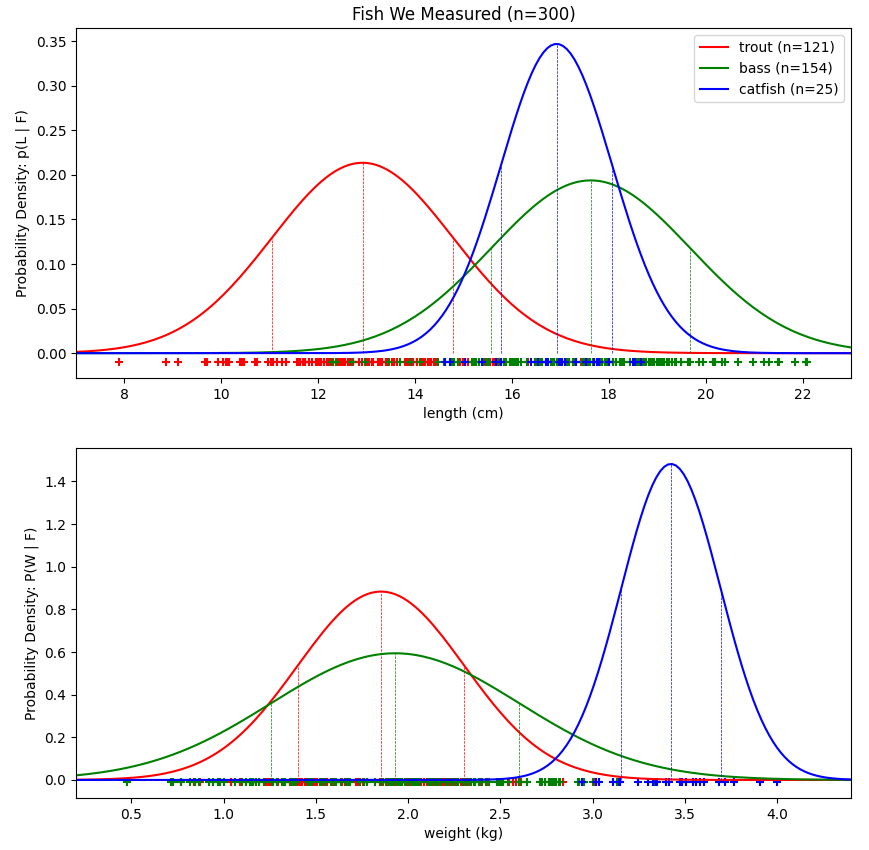
\includegraphics[width=0.7\textwidth]{2_unip.png}

(Source:\texttt{2\_univariates.py})

Note that the area under each one of those curves is exactly 1.0.  They are probability distributions.

Now we can use the formula for the normal distribution:

$$p(x) = \frac{1}{\sqrt{2\pi\sigma^2}} e^{-\frac{(x - \mu)^2}{2\sigma^2}}$$

Thus,

\begin{tabular}{c | c | c }
Given & $p(L=16 | F)$ & $p(W=2.1 | F)$ \\
\hline
$F$=Trout & .0546  & .7607 \\
$F$=Bass &  .1418 &.5753 \\
$F$=Catfish  & .2516 & 0.01 \\
\end{tabular}

Now, using the naive assumption, we can compute the joint probability for any type of fish: 

$$p(F=?, L=16 , W=2.1) = p(W=2.1 | F=?) p(L=16 | F=?)p(F=?)$$

\begin{tabular}{c | c }
For & $p(L=16, W=2.1, F=?)$ \\
\hline
$F$=Trout & .016763\\
$F$=Bass &  .041886  \\
$F$=Catfish  &  0.00001\\
\end{tabular}

The sum of these is $p(L=16, W=2.1)$: $.0586$

By the definition of conditional probability:

$$p(F=? | L=16, W=2.1) = \frac{p(F=?, L=16, W=2.1) }{p(L=16, W=2.1)}$$

So

\begin{tabular}{c | c }
For & $p(F=? | L=16, W=2.1)$ \\
\hline
$F$=Trout & .286\\
$F$=Bass &  .714  \\
$F$=Catfish  &  $\approx 0$\\
\end{tabular}

If you pull a random fish out of the lake and its length is 16 and its weight is 2.1, there is a 71.4\% chance that it is bass.  There is a 28.6\% chance it is a trout.

\section{Using the multivariate Gaussian distribution}

Give the kind of fish, length and width are independent!?  That makes no sense.  Longer fish tend to be heavier, right?

The multivariate Gaussian distribution is a generalization of the normal distribution::
\begin{itemize}
\item It deals with data of any dimension $d$.
\item It can includes the idea of covariance: For example, length and width are not independent.
\end{itemize}

If we use your naive Bayes,  we can get two dimensional density plots that would look like this:

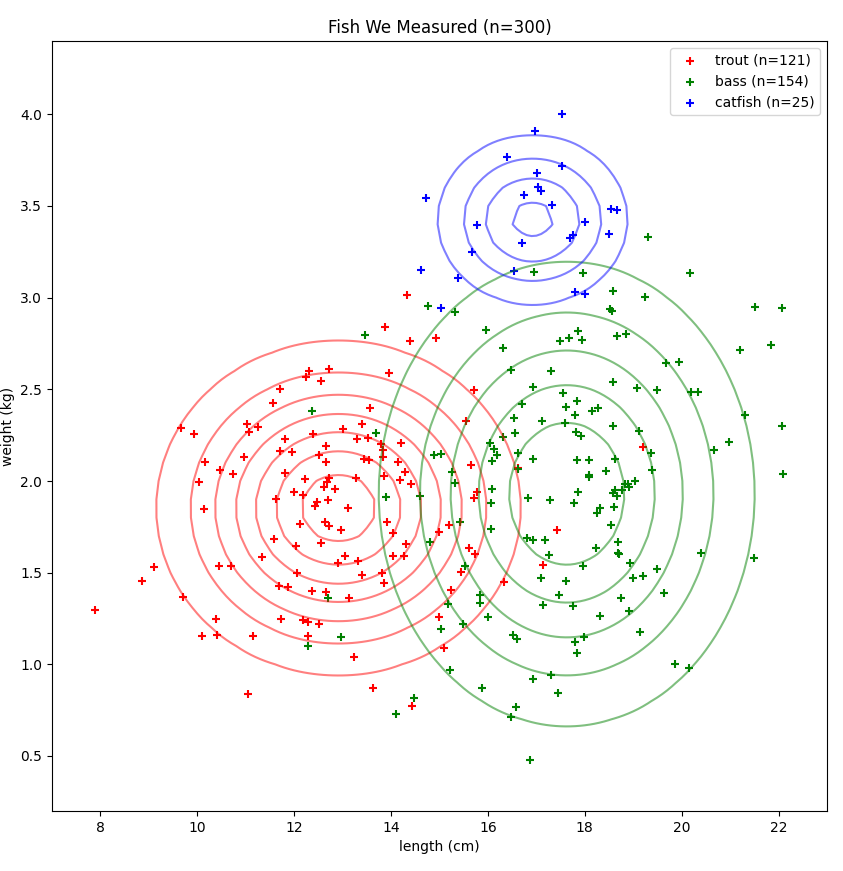
\includegraphics[width=0.55\textwidth]{4_indep_density.png}

With independence,   the ovals are circles,  ovals that go up, or ovals that sideways.  If we use the multivariate Gaussian distribution, we get:

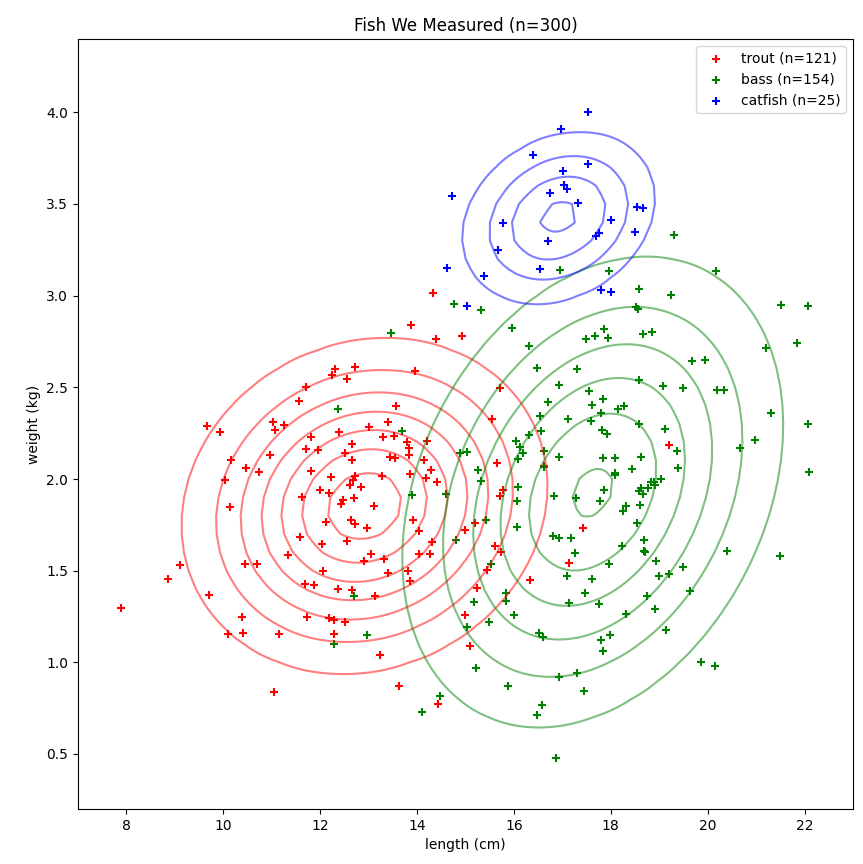
\includegraphics[width=0.55\textwidth]{5_full.png}

When there is covariance,  the ovals can slant in any direction.

If we discard the naive assumption,  we should get slightly more accurate results.

The multivariate Gaussian distribution uses vectors and matrices.  The mean $\vec{\mu}$ is a vector of dimension $d$.    The variance of each variable and its covariance with the other variables is captured in a $d \times d$ matrix called \textit{the covariance matrix} usually called $\boldsymbol\Sigma$.  (Yes, this is also the symbol for summation.  This creates some confusion at times, but you can usually figure out which is intended by the context.)

When you know $\vec{\mu}$ and $\boldsymbol\Sigma$,  the probability density for any vector $\vec{x}$ is:

$$p(\vec{x}) = (2\pi)^{-d/2}\det (\boldsymbol\Sigma)^{-1/2} \, \exp \left( -\frac{1}{2} (\vec{x} - \vec\mu)^\mathrm{T} \boldsymbol\Sigma^{-1}(\vec{x} - \vec\mu) \right)$$

If I have a bunch of data points $\vec{x_1}, ..., \vec{x_n}$.   How do I compute the values of $\vec{\mu}$ and $\boldsymbol\Sigma$ for which the observations $\vec{x_1}, ..., \vec{x_n}$ would be most likely?

$$\vec{\mu} = \frac{1}{n} \sum_{i = 1}^{d} \vec{x_i}$$

And the covariance matrix?  (Here we think of each $\vec{x_i}$  and $\vec{\mu}$ as  column vectors.)

$$\boldsymbol\Sigma = \frac{1}{n}\sum_{i=1}^n (\vec{x}_i-\vec{\mu})(\vec{x}_i-\vec{\mu})^\mathrm{T}$$

Notice that the diagonal entries of the matrix are the variance of each variable.  Notice also, that this is a symmetric matrix.

Applying this to our data we get:


\begin{tabular}{c | c | c}
Fish & $\vec{\mu}$  &$\boldsymbol\Sigma$ \\
\hline   & &\\
Trout & $\begin{bmatrix}
 12.91522571\\1.85290281
 \end{bmatrix}$ & 
$\begin{bmatrix}
3.51963149 & 0.09975744 \\
 0.09975744, & 0.20557471
 \end{bmatrix}$ \\ & & \\
Bass  & $\begin{bmatrix}
  17.62628327 \\ 1.92960088
 \end{bmatrix}$ & 
$\begin{bmatrix}
4.26652216 & 0.39553268 \\
0.39553268 & 0.45387711
 \end{bmatrix}$\\ & & \\
 
 Catfish  & $\begin{bmatrix}16.92187387 \\ 3.42423185
 \end{bmatrix}$ & 
$\begin{bmatrix}
1.37814515 &0.07281453 \\
0.07281453 & 0.07546403
 \end{bmatrix}$\\
\end{tabular}

We can use these to compute the likelihood of seeing a fish with length = 16 and weight = 2.1 for each type of fish:

\begin{tabular}{c | c }
Given & $p(L=16, W=2.1 | F=?)$ \\
\hline
$F$=Trout & .04578 \\
$F$=Bass &  .07732 \\
$F$=Catfish  & .000001 
\end{tabular}

Multiplied by the prior to get the joint probability:

\begin{tabular}{c | c }
Given & $p(L=16, W=2.1, F=?)$ \\
\hline
$F$=Trout & .01847 \\
$F$=Bass &  .03969 \\
$F$=Catfish  &  $\approx 0$
\end{tabular}

We sum those to get $p(L=16, W=2.1) = .0582$

\begin{tabular}{c | c }
Given & $p(F=? | L=16, W=2.1)$ \\
\hline
$F$=Trout & .318 \\
$F$=Bass &  .682 \\
$F$=Catfish  &  $\approx 0$
\end{tabular}

Given a randomly selected fish that is 19 inches long and 2.1 kg in weight,  you would guess that it is a bass with a confidence of 68.2\%.


